\documentclass[12pt]{article}
%%%%%%%%%%%%%%%%%
\author{Kristina Yancey Spencer}
\title{Survey of Optimization Methodologies Used in Combinatorial Nuclear Studies}

%%%% packages and definitions
\usepackage[style=ieee,backend=bibtex8,sorting=none]{biblatex}
\usepackage{color}
\usepackage{datetime}
\usepackage{gensymb}
\usepackage[letterpaper]{geometry}
\usepackage{graphicx}
\usepackage{pdflscape}
\usepackage{placeins}
\usepackage[doublespacing]{setspace}
\usepackage{textcomp}
\usepackage{titlesec}
\usepackage[table]{xcolor}

\bibliography{studies.bib}
\definecolor{taupe}{RGB}{227,227,218}
\definecolor{midnight}{RGB}{31,26,59}
\definecolor{darkblue}{RGB}{48,53,97}
\definecolor{medblue}{RGB}{111,129,173}
\definecolor{lightblue}{RGB}{162,179,207}
\definecolor{grey}{RGB}{212,217,219}
\definecolor{lightgrey}{RGB}{233,236,237}
\geometry{verbose,tmargin=1.25in,bmargin=1.25in,lmargin=1.4in,rmargin=1.15in}
  
%%%% formatting
\titleformat{\section}
  {\normalfont\fontsize{14}{15}\bfseries}{\thesection}{1em}{}
\titleformat{\subsection}
  {\normalfont\fontsize{12}{15}\bfseries}{\thesubsection}{1em}{}
\setlength{\parskip}{1em} % Single-space between paragraphs
\renewcommand{\baselinestretch}{1.0} % single spacing lines
\newdate{date}{21}{03}{2016}
\date{\displaydate{date}}
   
% =======================================================================
\begin{document}
\maketitle

The journal articles included in this PDF were found during the literature review for the dissertation, \textit{Adaptable Long-term Optimization of Dry Cask Storage Loading Patterns}. This survey was conducted to determine which optimization algorithms nuclear engineers have used to solve combinatorial problems. The survey was conducted using three searches:
\begin{enumerate}
	\item Science Direct: ``in-core shuffle,'' 
	\item Science Direct: ``nuclear optimization,''
	\item American Nuclear Society: ``optimization.''
\end{enumerate}
During the search, journal articles about continuous problems were ignored, and the search was conducted until 100 papers had been surveyed. This PDF categorizes the studies and includes some notes that were taken down during the search.

\begin{figure}
	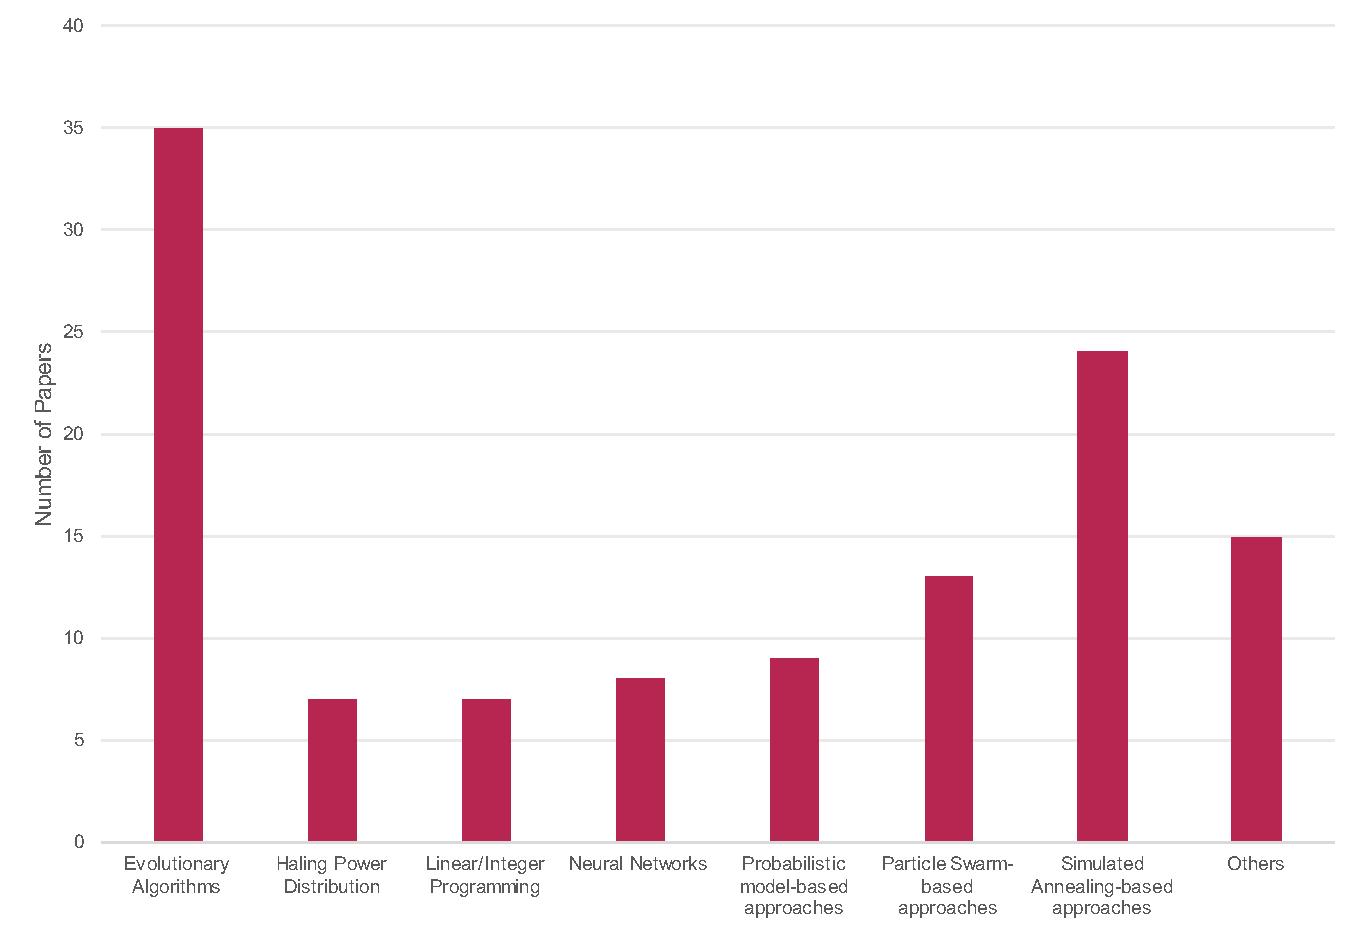
\includegraphics[width=\textwidth]{methods1}
	\caption{Distribution of optimization methodologies used for combinatorial problems in nuclear engineering. This table was created based on a survey of 100 papers: \cite{Haling:1964,Wall:1965,Sauar:1971,Miller:1975,Motoda:1975,Comes:1988,Okafor:1988,Stillman:1989,Burte:1993,Mahlers:1994,Smuc:1994,Feltus:1995,Stevens:1995,DeChaine:1996,Axmann:1997,Kim:1997,Mahlers:1997,Yamamoto:1997,Lin:1998,Chapot:1999,Francois:1999,Moore:1999,Toshinsky:1999,Karve:2000,Yamamoto:2000,Hongchun:2001,Jagawa:2001,Lee:2001,Kobayashi:2002,Machado:2002,Erdoan:2003,Faria:2003,Sadighi:2003,Yamamoto:2003,Alim:2004,Alim:2004a,Guler:2004,Ortiz:2004,Yamamoto:2004,Ziver:2004,Alim:2005,Francois:2005,Keller:2005,Do:2006,Wang:2006,Castillo:2007,Francois:2007,Hadavi:2007,Hernandez:2007,Keller:2007,Kim:2007,Lima:2007,Park:2007,Alim:2008,Fadaei:2008,Lima:2008,Park:2008,De-Moura-Meneses:2009,Waintraub:2009,Zerovnik:2009,De-Moura-Meneses:2010,Ishida:2010,Shaukat:2010,Zio:2010,Hays:2011,Kropaczek:2011,Norouzi:2011,Oliveira:2011,Ortiz-Servin:2011,Silva:2011,Silva:2011a,Tsvetkov:2011,Yadav:2011,Carlos:2012,Hays:2012,Lin:2012,Liu:2012,Aghaie:2013,Kropaczek:2013,Levine:2013,Wang:2013,Arshi:2014,Carlsen:2014,Hedayat:2014,Khoshahval:2014,Khoshahval:2014a,Lin:2014,Park:2014,Silva:2014,Zameer:2014,Camara-Augusto:2015,De-Moura-Meneses:2015,Hill:2015,Ottinger:2015,Park:2015,Poursalehi:2015,Su:2015,Ayoobian:2016,Hou:2016,Schlunz:2016}.}
	\label{fig:method1}
\end{figure}


\begin{figure}
	\centering
	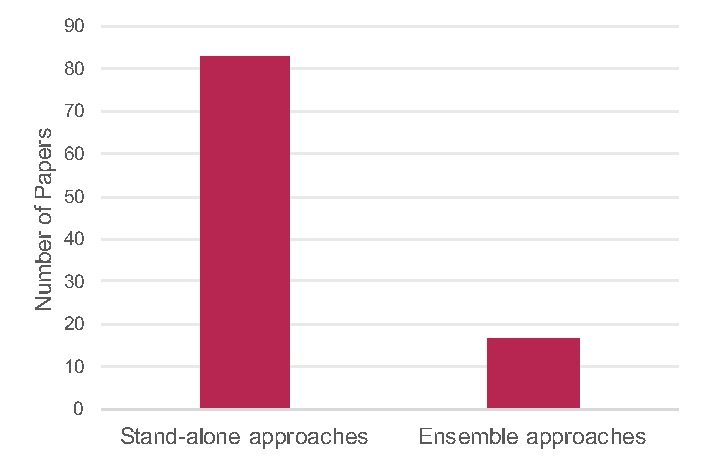
\includegraphics[width=0.6\textwidth]{methods2}
	\caption{Comparison of stand-alone versus ensemble optimization approaches in nuclear engineering. This table was created based on a survey of 100 papers: \cite{Haling:1964,Wall:1965,Sauar:1971,Miller:1975,Motoda:1975,Comes:1988,Okafor:1988,Stillman:1989,Burte:1993,Mahlers:1994,Smuc:1994,Feltus:1995,Stevens:1995,DeChaine:1996,Axmann:1997,Kim:1997,Mahlers:1997,Yamamoto:1997,Lin:1998,Chapot:1999,Francois:1999,Moore:1999,Toshinsky:1999,Karve:2000,Yamamoto:2000,Hongchun:2001,Jagawa:2001,Lee:2001,Kobayashi:2002,Machado:2002,Erdoan:2003,Faria:2003,Sadighi:2003,Yamamoto:2003,Alim:2004,Alim:2004a,Guler:2004,Ortiz:2004,Yamamoto:2004,Ziver:2004,Alim:2005,Francois:2005,Keller:2005,Do:2006,Wang:2006,Castillo:2007,Francois:2007,Hadavi:2007,Hernandez:2007,Keller:2007,Kim:2007,Lima:2007,Park:2007,Alim:2008,Fadaei:2008,Lima:2008,Park:2008,De-Moura-Meneses:2009,Waintraub:2009,Zerovnik:2009,De-Moura-Meneses:2010,Ishida:2010,Shaukat:2010,Zio:2010,Hays:2011,Kropaczek:2011,Norouzi:2011,Oliveira:2011,Ortiz-Servin:2011,Silva:2011,Silva:2011a,Tsvetkov:2011,Yadav:2011,Carlos:2012,Hays:2012,Lin:2012,Liu:2012,Aghaie:2013,Kropaczek:2013,Levine:2013,Wang:2013,Arshi:2014,Carlsen:2014,Hedayat:2014,Khoshahval:2014,Khoshahval:2014a,Lin:2014,Park:2014,Silva:2014,Zameer:2014,Camara-Augusto:2015,De-Moura-Meneses:2015,Hill:2015,Ottinger:2015,Park:2015,Poursalehi:2015,Su:2015,Ayoobian:2016,Hou:2016,Schlunz:2016}}
	\label{fig:method2}
\end{figure}


\begin{landscape}
\begin{table}
	\rowcolors{2}{white}{lightgrey}
	\singlespacing
	\footnotesize
\begin{tabular}{  p{0.28\linewidth} p{0.3\linewidth} p{0.3\linewidth} p{0.1\linewidth} }
 \hline
 &  \textbf{Pros}  & \textbf{Cons} & \textbf{References} \\
 \hline
 
 \textbf{Biogeography} & & & \textcolor{medblue}{\cite{Khoshahval:2014}} \\
 
 \textbf{Genetic Algorithm} & \textcolor{medblue}{well known, widely used (MATLAB), flexible, robust, good exploration abilities} & \textcolor{medblue}{poor local search ability} & \textcolor{medblue}{\cite{DeChaine:1996,Hadavi:2007,Chapot:1999,Shaukat:2010,Norouzi:2011,Toshinsky:1999,Hongchun:2001,Ayoobian:2016,Zio:2010,Keller:2005,Keller:2007,Carlsen:2014,Alim:2004,Alim:2005,Do:2006,Alim:2004a,Yamamoto:1997,Kobayashi:2002,Axmann:1997,Erdoan:2003,Ziver:2004,Alim:2008,Levine:2013,Zameer:2014,Wang:2006}} \\
 
 \textbf{Harmony Search Algorithms} &  &  & \textcolor{medblue}{\cite{Aghaie:2013,Schlunz:2016}} \\
 
 \textbf{Quantum Population-Based Incremental Learning Algorithm} & \textcolor{medblue}{} & \textcolor{medblue}{} & \textcolor{medblue}{\cite{Silva:2011,Silva:2014}}  \\
 
 \textbf{Shuffled Frog Leaping Algorithm} & \textcolor{medblue}{} & \textcolor{medblue}{} & \textcolor{medblue}{\cite{Arshi:2014}} \\
 
 \hline
\end{tabular}
\caption{Evolutionary Algorithms}\label{table:evolalg} 
\end{table}
\end{landscape}


\begin{landscape}
\begin{table}
	\rowcolors{2}{white}{lightgrey}
	\singlespacing
	\footnotesize
\begin{tabular}{  p{0.2\linewidth} p{0.34\linewidth} p{0.34\linewidth} p{0.1\linewidth} }
 \hline
 &  \textbf{Pros}  & \textbf{Cons} & \textbf{References} \\
 \hline
 
 \textbf{Artificial Bee Colony} & \textcolor{medblue}{powerful global search ability, fewer control parameters to tune than GA or PSO} & \textcolor{medblue}{poor local search ability} &  \textcolor{medblue}{\cite{Oliveira:2011}} \\
 
 \textbf{Firefly Algorithm} & & & \textcolor{medblue}{\cite{Poursalehi:2015}} \\
 
 \textbf{Particle Swarm Optimization} & \textcolor{medblue}{powerful local search ability, faster than other evolutional algorithms} & \textcolor{medblue}{poor global search ability} & \textcolor{medblue}{\cite{Yadav:2011,Wang:2013,Waintraub:2009,Carlos:2012,Camara-Augusto:2015,De-Moura-Meneses:2009,Zameer:2014,De-Moura-Meneses:2010,Khoshahval:2014a}} \\
 
 \textbf{Improved Pivot Particle Swarm Optimization} & \textcolor{medblue}{PSO + better global searching} & \textcolor{medblue}{not stated - wonder if HPA or IPPSO improves more?} & \textcolor{medblue}{\cite{Liu:2012}} \\
 
 \textbf{Shuffled Frog Leaping Algorithm} & & & \textcolor{medblue}{\cite{Arshi:2014}} \\
 
 \hline
\end{tabular}
\caption{Particle Swarm-based Approaches}\label{table:pso} 
\end{table}

\begin{table}
	\rowcolors{2}{white}{lightgrey}
	\singlespacing
	\footnotesize
\begin{tabular}{  p{0.2\linewidth} p{0.34\linewidth} p{0.34\linewidth} p{0.1\linewidth} }
 \hline
 &  \textbf{Pros}  & \textbf{Cons} & \textbf{References} \\
 \hline
 
 \textbf{Ant Colony Algorithms} & \textcolor{medblue}{efficient and versatile for combinatorial problems} & & \textcolor{medblue}{\cite{Lin:2012,Machado:2002,Lima:2007,Lima:2008,Lin:2014,Silva:2011a}} \\
 
 \textbf{Cross Entropy} & \textcolor{medblue}{} & \textcolor{medblue}{} & \textcolor{medblue}{\cite{De-Moura-Meneses:2015}} \\
 
 \textbf{Quantum Population-Based Incremental Learning Algorithm} & \textcolor{medblue}{} & \textcolor{medblue}{} &  \textcolor{medblue}{\cite{Silva:2011,Silva:2011a,Silva:2014}} \\
 
 \hline
\end{tabular}
\caption{Probabilistic model-based approaches}\label{table:probmethod} 
\end{table}
\end{landscape}


\begin{landscape}
\begin{table}
	\rowcolors{2}{white}{lightgrey}
	\singlespacing
	\footnotesize
\begin{tabular}{  p{0.2\linewidth} p{0.34\linewidth} p{0.34\linewidth} p{0.1\linewidth} }
 \hline
 &  \textbf{Pros}  & \textbf{Cons} & \textbf{References} \\
 \hline
 
 \textbf{Artificial Neural Networks} & \textcolor{medblue}{robust, does not need to pre-fix algorithm parameters, possibly faster} & \textcolor{medblue}{training stage may not converge, generalization ability can be a problem} & \textcolor{medblue}{\cite{Faria:2003,Ortiz:2004,Ortiz-Servin:2011,Yamamoto:2003,Erdoan:2003,Ziver:2004,Sadighi:2003,Fadaei:2008}} \\
 
 \textbf{Haling Power Distribution} & & & \textcolor{medblue}{\cite{Guler:2004,Feltus:1995,Burte:1993,Haling:1964,Alim:2008,Levine:2013}} \\
 
 \textbf{Heuristics} & \textcolor{medblue}{fast, intuitive, gives verifiable results} & \textcolor{medblue}{always an example that causes the algorithm to fail} & \textcolor{medblue}{\cite{Zerovnik:2009,Francois:1999,Kim:2007,Tsvetkov:2011}} \\
 
 \textbf{Linear Programming} & \textcolor{medblue}{relatively simple and scalable} & \textcolor{medblue}{the problem needs to be linear and certain, decision variables need to be independent} & \textcolor{medblue}{\cite{Miller:1975,Okafor:1988,Stillman:1989,Motoda:1975,Mahlers:1997,Kim:1997}} \\
 
 \textbf{Monte Carlo Integer Programming} & \textcolor{medblue}{able to handle a large number of decision variables, does not require everything to be linearized, determines not only optimal solution but also near-optimum family of solutions} & \textcolor{medblue}{not stated} & \textcolor{medblue}{\cite{Comes:1988}}  \\
 
 \textbf{Simulated Annealing} & \textcolor{medblue}{able to optimize over large search spaces and to handle many local optima; able to handle nonlinear objectives and constraints combined with discrete variables} & \textcolor{medblue}{if cooling schedule too fast, solution may be trapped in local minimum, too slow, low computational efficiency} & \textcolor{medblue}{\cite{Smuc:1994,Moore:1999,Karve:2000,Hays:2011,Hays:2012,Kropaczek:2013,Hou:2016,Mahlers:1994,Hedayat:2014,Ottinger:2015,Kropaczek:2011,Yamamoto:2004,Park:2007,Hernandez:2007,Park:2008,Park:2015,Lee:2001,Park:2014,Yamamoto:2000,Stevens:1995,Su:2015,Sadighi:2003,Fadaei:2008,Khoshahval:2014a}} \\
 
 \textbf{The Tabu Search} & & & \textcolor{medblue}{\cite{Castillo:2007,Hill:2015,Lin:1998,Jagawa:2001,Wang:2006,Lin:2014}} \\
 
 \hline
\end{tabular}
\caption{Optimization Methodologies}\label{table:optimethod} 
\end{table}
\end{landscape}

Nuclear articles with hybrid methods:
\begin{itemize}
	\item Ant Colony + Tabu Hybrid: \cite{Lin:2014}
	\item Artificial Neural Network + Genetic Algorithm: \cite{Erdoan:2003,Ziver:2004}
	\item Artificial Neural Network + Simulated Annealing: \cite{Sadighi:2003,Fadaei:2008}
	\item Genetic Algorithm + Haling Power Distribution: \cite{Alim:2008,Levine:2013}
	\item Genetic Algorithm + Simulated Annealing: \cite{Zameer:2014}
	\item Genetic Algorithm + Tabu Search: \cite{Wang:2006}
	\item Particle Swarm Optimization + Heuristics: \cite{De-Moura-Meneses:2010}
	\item Particle Swarm Optimization + Local Search: Liu and Cai incorporate the M. Clerc pivot local search method with PSO to improve the local search ability for a fuel loading pattern optimization study in~\cite{Liu:2012}.
	\item Particle Swarm Optimization + Simulated Annealing: \cite{Khoshahval:2014a}
	\item Quantum Population-Based Incremental Learning Algorithm: \cite{Silva:2011,Silva:2014}
	\item Quantum + Ant Colony: \cite{Silva:2011a}
	\item Simulated Annealing + Branch \& Bound: \cite{Su:2015}
	\item Shuffled Frog Leaping: Ensemble of particle swarm optimization and the shuffled complex evolution technique in~\cite{Arshi:2014}.
\end{itemize}

%%%%%%%%%%%%%%%%%%%%%%%%%%%%%%%%%%%%%%%%%%%%%%%%%%%%%%%%%%%%%%%%%%%%%%%%%

\FloatBarrier
\printbibliography

\end{document}